\documentclass{article}
\usepackage{graphicx}
\usepackage{amssymb,amsmath}
\usepackage{tikz}
\usepackage{pgfplots}
\pgfplotsset{compat=newest}
\pgfplotsset{plot coordinates/math parser=false}
\newlength\figureheight
\newlength\figurewidth
\usetikzlibrary{shapes, arrows, patterns, external}

\DeclareRobustCommand{\BlackBox}{\State \textbf{Black Box: }}
\DeclareRobustCommand{\Test}{\State \textbf{Test: }}
\DeclareRobustCommand{\Define}{\State \textbf{Define: }}
\DeclareRobustCommand{\Update}{\State \textbf{Update: }}
\DeclareRobustCommand{\Set}{\State \textbf{Set: }}
\DeclareRobustCommand{\Calculate}{\State \textbf{Calculate: }}
%\newcommand{\algorithmicset}{\textbf{Set:}}
%\algnewcommand\Solve{\item[\algorithmicset]}
%============================================================================
% commands.tex
%============================================================================
% This file contains:
% 	- Defined Variables
%	- Redefined math shorthand
%	- Defined math shorthand

%============================================================================
% Defined Variables
%============================================================================
% 	- \abstractType:
%		Use: Toggles the type of abstract to be used
%		Default Value: abstract
%		Options: abstract, umiabstract
\newcommand{\abstractType}{abstract}

%============================================================================
% Redefined Math Commands
%============================================================================
% 	- \Vec{1} or \vec{1}
%		Long Name: Vector
%		Arguements[1]: bold and overbar arg1	
\DeclareRobustCommand{\Vec}[1]{%
    \ifmmode
        \mathbf{#1}\,%
    \else
        $\displaystyle \mathbf{#1}\,$%
    \fi
}
\DeclareRobustCommand{\vec}[1]{\Vec{#1}}

\DeclareRobustCommand{\lbm}{%
    \ifmmode
        \text{lb}_{\text{m}}
    \else
        $\displaystyle \text{lb}_{\text{m}}$%
    \fi
}
\DeclareRobustCommand{\lbf}{%
    \ifmmode
        \text{lb}_{\text{f}}
    \else
        $\displaystyle \text{lb}_{\text{f}}$
    \fi
}
\DeclareRobustCommand{\dt}{%
	\ifmmode
		\Delta t
	\else
		$Delta t$
	\fi
}
\DeclareRobustCommand{\dtmax}{%
	\ifmmode
		\Delta t_{\text{MAX}}
	\else
		$\Delta t_{\text{MAX}}$
	\fi
}
\DeclareRobustCommand{\dx}{%
	\ifmmode
		\Delta x
	\else
		$\Delta x$
	\fi
}

\delimitershortfall-1sp
\newcommand\abs[1]{\left|#1\right|}

\tikzstyle{Decision} = [diamond, draw, text width=4.5em, text badly centered, node distance=3cm, inner sep=0pt]
\tikzstyle{Action} = [rectangle, draw,text width=5em, text centered, node distance=3cm, rounded corners, minimum height=0em]
\tikzstyle{NodePoint} = [circle, draw, minimum height = 0 em, node distance = 3 cm]
\tikzstyle{BlackBox} = [rectangle, draw, text centered, node distance=1cm, fill=black!10]
\tikzstyle{line} = [draw, -latex']
    
\begin{document}

\begin{figure}
\centering
% This file was created by matlab2tikz v0.4.2.
% Copyright (c) 2008--2013, Nico Schlömer <nico.schloemer@gmail.com>
% All rights reserved.
% 
% The latest updates can be retrieved from
%   http://www.mathworks.com/matlabcentral/fileexchange/22022-matlab2tikz
% where you can also make suggestions and rate matlab2tikz.
% 
% 
% 
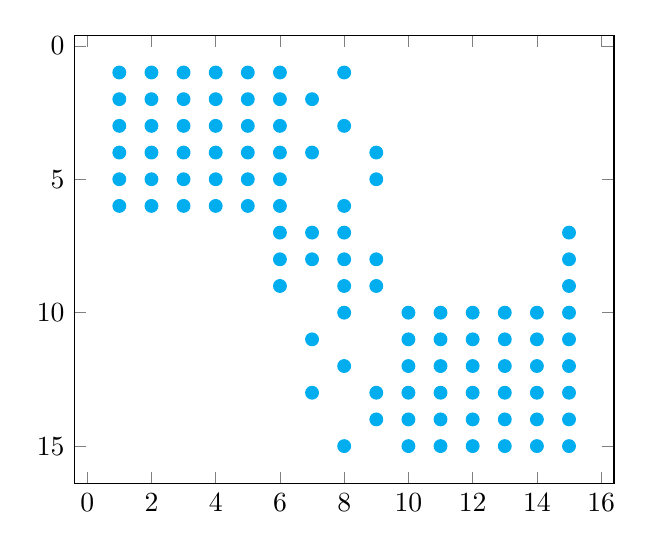
\begin{tikzpicture}

\begin{axis}[%
%width=4.52083333333333in,
%height=3.565625in,
%scale only axis,
%xmin=0,
%xmax=16,
%xlabel={nz = 99},
y dir=reverse,
%ymin=0,
%ymax=16
]
\addplot [
color=cyan,
mark size=2.3pt,
only marks,
mark=*,
mark options={solid},
forget plot
]
table[row sep=crcr]{
1 1\\
1 2\\
1 3\\
1 4\\
1 5\\
1 6\\
2 1\\
2 2\\
2 3\\
2 4\\
2 5\\
2 6\\
3 1\\
3 2\\
3 3\\
3 4\\
3 5\\
3 6\\
4 1\\
4 2\\
4 3\\
4 4\\
4 5\\
4 6\\
5 1\\
5 2\\
5 3\\
5 4\\
5 5\\
5 6\\
6 1\\
6 2\\
6 3\\
6 4\\
6 5\\
6 6\\
6 7\\
6 8\\
6 9\\
7 2\\
7 4\\
7 7\\
7 8\\
7 11\\
7 13\\
8 1\\
8 3\\
8 6\\
8 7\\
8 8\\
8 9\\
8 10\\
8 12\\
8 15\\
9 4\\
9 5\\
9 8\\
9 9\\
9 13\\
9 14\\
10 10\\
10 11\\
10 12\\
10 13\\
10 14\\
10 15\\
11 10\\
11 11\\
11 12\\
11 13\\
11 14\\
11 15\\
12 10\\
12 11\\
12 12\\
12 13\\
12 14\\
12 15\\
13 10\\
13 11\\
13 12\\
13 13\\
13 14\\
13 15\\
14 10\\
14 11\\
14 12\\
14 13\\
14 14\\
14 15\\
15 7\\
15 8\\
15 9\\
15 10\\
15 11\\
15 12\\
15 13\\
15 14\\
15 15\\
};
%\addplot [
%color=blue,
%mark size=2.3pt,
%only marks,
%mark=*,
%mark options={solid},
%forget plot
%]
%table[row sep=crcr]{
%8 1\\
%};
\end{axis}
\end{tikzpicture}%
\end{figure}

\begin{figure}
\centering
% This file was created by matlab2tikz v0.4.2.
% Copyright (c) 2008--2013, Nico Schlömer <nico.schloemer@gmail.com>
% All rights reserved.
% 
% The latest updates can be retrieved from
%   http://www.mathworks.com/matlabcentral/fileexchange/22022-matlab2tikz
% where you can also make suggestions and rate matlab2tikz.
% 
% 
% 
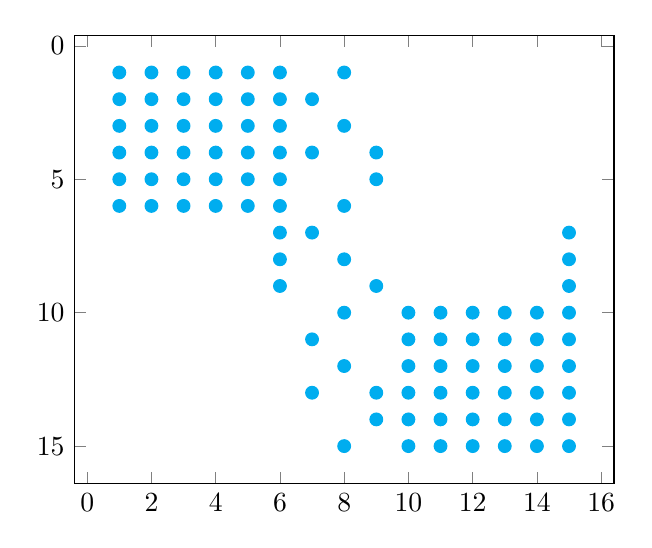
\begin{tikzpicture}

\begin{axis}[%
%width=4.52083333333333in,
%height=3.565625in,
%scale only axis,
%xmin=0,
%xmax=16,
%xlabel={nz = 99},
y dir=reverse,
%ymin=0,
%ymax=16
]
\addplot [
color=cyan,
mark size=2.3pt,
only marks,
mark=*,
mark options={solid},
forget plot
]
table[row sep=crcr]{
1 1\\
1 2\\
1 3\\
1 4\\
1 5\\
1 6\\
2 1\\
2 2\\
2 3\\
2 4\\
2 5\\
2 6\\
3 1\\
3 2\\
3 3\\
3 4\\
3 5\\
3 6\\
4 1\\
4 2\\
4 3\\
4 4\\
4 5\\
4 6\\
5 1\\
5 2\\
5 3\\
5 4\\
5 5\\
5 6\\
6 1\\
6 2\\
6 3\\
6 4\\
6 5\\
6 6\\
6 7\\
6 8\\
6 9\\
7 2\\
7 4\\
7 7\\
7 11\\
7 13\\
8 1\\
8 3\\
8 6\\
8 8\\
8 10\\
8 12\\
8 15\\
9 4\\
9 5\\
9 9\\
9 13\\
9 14\\
10 10\\
10 11\\
10 12\\
10 13\\
10 14\\
10 15\\
11 10\\
11 11\\
11 12\\
11 13\\
11 14\\
11 15\\
12 10\\
12 11\\
12 12\\
12 13\\
12 14\\
12 15\\
13 10\\
13 11\\
13 12\\
13 13\\
13 14\\
13 15\\
14 10\\
14 11\\
14 12\\
14 13\\
14 14\\
14 15\\
15 7\\
15 8\\
15 9\\
15 10\\
15 11\\
15 12\\
15 13\\
15 14\\
15 15\\
};
%\addplot [
%color=blue,
%mark size=2.3pt,
%only marks,
%mark=*,
%mark options={solid},
%forget plot
%]
%table[row sep=crcr]{
%8 1\\
%};
\end{axis}
\end{tikzpicture}%
\end{figure}

\begin{figure}
\centering
% This file was created by matlab2tikz v0.4.2.
% Copyright (c) 2008--2013, Nico Schlömer <nico.schloemer@gmail.com>
% All rights reserved.
% 
% The latest updates can be retrieved from
%   http://www.mathworks.com/matlabcentral/fileexchange/22022-matlab2tikz
% where you can also make suggestions and rate matlab2tikz.
% 
% 
% 
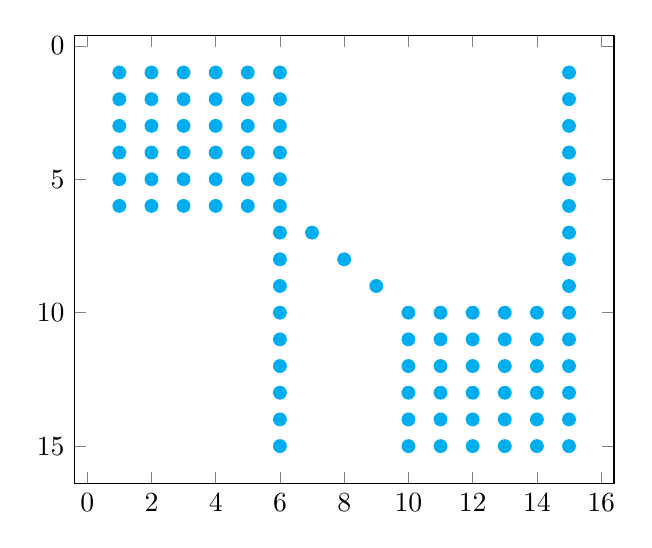
\begin{tikzpicture}

\begin{axis}[%
%width=4.52083333333333in,
%height=3.565625in,
%scale only axis,
%xmin=0,
%xmax=16,
%xlabel={nz = 99},
y dir=reverse,
%ymin=0,
%ymax=16
]
\addplot [
color=cyan,
mark size=2.3pt,
only marks,
mark=*,
mark options={solid},
forget plot
]
table[row sep=crcr]{
1 1\\ 2 1\\ 3 1\\ 4 1\\ 5 1\\ 6 1\\ 15 1\\
%
1 2\\ 2 2\\ 3 2\\ 4 2\\ 5 2\\ 6 2\\ 15 2\\
%
1 3\\ 2 3\\ 3 3\\ 4 3\\ 5 3\\ 6 3\\ 15 3\\
%
1 4\\ 2 4\\ 3 4\\ 4 4\\ 5 4\\ 6 4\\ 15 4\\
%
1 5\\ 2 5\\ 3 5\\ 4 5\\ 5 5\\ 6 5\\ 15 5\\
%
1 6\\ 2 6\\ 3 6\\ 4 6\\ 5 6\\ 6 6\\ 15 6\\
%
6 7\\ 7 7\\ 15 7\\
%
6 8\\ 8 8\\ 15 8\\
%
6 9\\ 9 9\\ 15 9\\
%
6 10\\ 10 10\\ 11 10\\ 12 10\\ 13 10\\ 14 10\\ 15 10\\
%
6 11\\ 10 11\\ 11 11\\ 12 11\\ 13 11\\ 14 11\\ 15 11\\
%
6 12\\ 10 12\\ 11 12\\ 12 12\\ 13 12\\ 14 12\\ 15 12\\
%
6 13\\ 10 13\\ 11 13\\ 12 13\\ 13 13\\ 14 13\\ 15 13\\
%
6 14\\ 10 14\\ 11 14\\ 12 14\\ 13 14\\ 14 14\\ 15 14\\
%
6 15\\ 10 15\\ 11 15\\ 12 15\\ 13 15\\ 14 15\\ 15 15\\
};
%\addplot [
%color=blue,
%mark size=2.3pt,
%only marks,
%mark=*,
%mark options={solid},
%forget plot
%]
%table[row sep=crcr]{
%8 1\\
%};
\end{axis}
\end{tikzpicture}%
\end{figure}

\begin{figure}
\centering
% This file was created by matlab2tikz v0.4.2.
% Copyright (c) 2008--2013, Nico Schlömer <nico.schloemer@gmail.com>
% All rights reserved.
% 
% The latest updates can be retrieved from
%   http://www.mathworks.com/matlabcentral/fileexchange/22022-matlab2tikz
% where you can also make suggestions and rate matlab2tikz.
% 
% 
% 
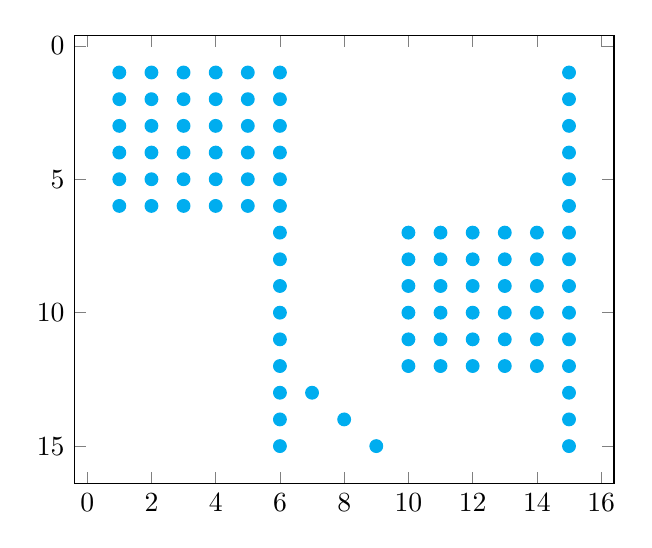
\begin{tikzpicture}

\begin{axis}[%
%width=4.52083333333333in,
%height=3.565625in,
%scale only axis,
%xmin=0,
%xmax=16,
%xlabel={nz = 99},
y dir=reverse,
%ymin=0,
%ymax=16
]
\addplot [
color=cyan,
mark size=2.3pt,
only marks,
mark=*,
mark options={solid},
forget plot
]
table[row sep=crcr]{
1 1\\ 2 1\\ 3 1\\ 4 1\\ 5 1\\ 6 1\\ 15 1\\
%
1 2\\ 2 2\\ 3 2\\ 4 2\\ 5 2\\ 6 2\\ 15 2\\
%
1 3\\ 2 3\\ 3 3\\ 4 3\\ 5 3\\ 6 3\\ 15 3\\
%
1 4\\ 2 4\\ 3 4\\ 4 4\\ 5 4\\ 6 4\\ 15 4\\
%
1 5\\ 2 5\\ 3 5\\ 4 5\\ 5 5\\ 6 5\\ 15 5\\
%
1 6\\ 2 6\\ 3 6\\ 4 6\\ 5 6\\ 6 6\\ 15 6\\
%
6 13\\ 7 13\\ 15 13\\
%
6 14\\ 8 14\\ 15 14\\
%
6 15\\ 9 15\\ 15 15\\
%
6 7 \\ 10 7 \\ 11 7 \\ 12 7 \\ 13 7 \\ 14 7 \\ 15 7 \\
%
6 8 \\ 10 8 \\ 11 8 \\ 12 8 \\ 13 8 \\ 14 8 \\ 15 8 \\
%
6 9 \\ 10 9 \\ 11 9 \\ 12 9 \\ 13 9 \\ 14 9 \\ 15 9 \\
%
6 10\\ 10 10\\ 11 10\\ 12 10\\ 13 10\\ 14 10\\ 15 10\\
%
6 11\\ 10 11\\ 11 11\\ 12 11\\ 13 11\\ 14 11\\ 15 11\\
%
6 12\\ 10 12\\ 11 12\\ 12 12\\ 13 12\\ 14 12\\ 15 12\\
};
%\addplot [
%color=blue,
%mark size=2.3pt,
%only marks,
%mark=*,
%mark options={solid},
%forget plot
%]
%table[row sep=crcr]{
%8 1\\
%};
\end{axis}
\end{tikzpicture}%
\end{figure}

\begin{figure}
\centering
% This file was created by matlab2tikz v0.4.2.
% Copyright (c) 2008--2013, Nico Schlömer <nico.schloemer@gmail.com>
% All rights reserved.
% 
% The latest updates can be retrieved from
%   http://www.mathworks.com/matlabcentral/fileexchange/22022-matlab2tikz
% where you can also make suggestions and rate matlab2tikz.
% 
% 
% 
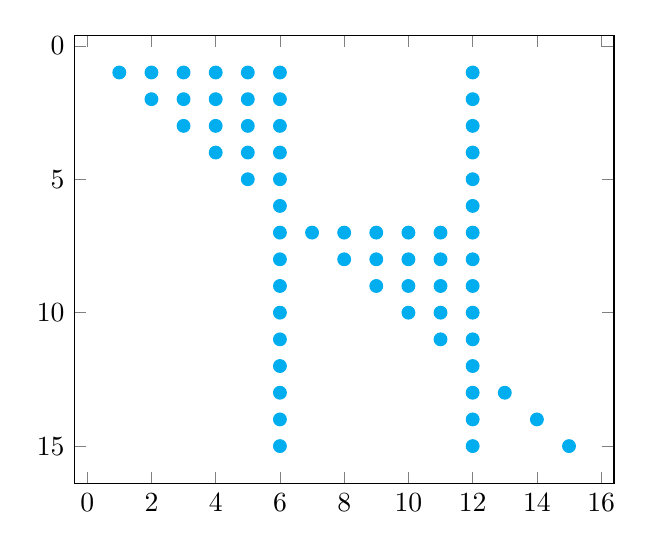
\begin{tikzpicture}

\begin{axis}[%
%width=4.52083333333333in,
%height=3.565625in,
%scale only axis,
%xmin=0,
%xmax=16,
%xlabel={nz = 99},
y dir=reverse,
%ymin=0,
%ymax=16
]
\addplot [
color=cyan,
mark size=2.3pt,
only marks,
mark=*,
mark options={solid},
forget plot
]
table[row sep=crcr]{
1 1\\ 2 1\\ 3 1\\ 4 1\\ 5 1\\ 6 1\\ 12 1\\
%
2 2\\ 3 2\\ 4 2\\ 5 2\\ 6 2\\ 12 2\\
%
3 3\\ 4 3\\ 5 3\\ 6 3\\ 12 3\\
%
4 4\\ 5 4\\ 6 4\\ 12 4\\
%
5 5\\ 6 5\\ 12 5\\
%
6 6\\ 12 6\\
%
6 13\\ 13 13\\ 12 13\\
%
6 14\\ 14 14\\ 12 14\\
%
6 15\\ 15 15\\ 12 15\\
%
6 7 \\  7 7 \\  8 7 \\ 9  7 \\ 10 7 \\ 11 7 \\ 12 7 \\
%
6 8 \\  8 8 \\ 9 8 \\ 10 8 \\ 11 8 \\ 12 8 \\
%
6 9 \\  9 9 \\ 10 9 \\ 11 9 \\ 12 9 \\
%
6 10\\  10 10\\ 11 10\\ 12 10\\
%
6 11\\  11 11\\ 12 11\\
%
6 12\\ 12 12\\
};
%\addplot [
%color=blue,
%mark size=2.3pt,
%only marks,
%mark=*,
%mark options={solid},
%forget plot
%]
%table[row sep=crcr]{
%8 1\\
%};
\end{axis}
\end{tikzpicture}%
\end{figure}

\begin{figure}
\centering
% This file was created by matlab2tikz v0.4.2.
% Copyright (c) 2008--2013, Nico Schlömer <nico.schloemer@gmail.com>
% All rights reserved.
% 
% The latest updates can be retrieved from
%   http://www.mathworks.com/matlabcentral/fileexchange/22022-matlab2tikz
% where you can also make suggestions and rate matlab2tikz.
% 
% 
% 
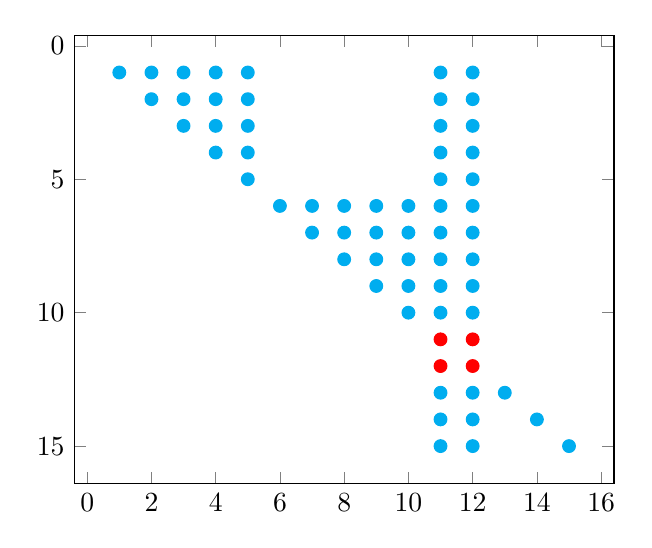
\begin{tikzpicture}

\begin{axis}[%
%width=4.52083333333333in,
%height=3.565625in,
%scale only axis,
%xmin=0,
%xmax=16,
%xlabel={nz = 99},
y dir=reverse,
%ymin=0,
%ymax=16
]
\addplot [
color=cyan,
mark size=2.3pt,
only marks,
mark=*,
mark options={solid},
forget plot
]
table[row sep=crcr]{
1 1\\ 2 1\\ 3 1\\ 4 1\\ 5 1\\ 11 1\\ 12 1\\
%
2 2\\ 3 2\\ 4 2\\ 5 2\\ 11 2\\ 12 2\\
%
3 3\\ 4 3\\ 5 3\\ 11 3\\ 12 3\\
%
4 4\\ 5 4\\ 11 4\\ 12 4\\
%
5 5\\ 11 5\\ 12 5\\
%
6 6 \\  7 6 \\  8 6 \\ 9  6 \\ 10 6 \\ 11 6 \\ 12 6 \\
%
7 7 \\  8 7 \\ 9 7 \\ 10 7 \\ 11 7 \\ 12 7 \\
%
8 8 \\  9 8 \\ 10 8 \\ 11 8 \\ 12 8 \\
%
9 9\\  10 9\\ 11 9\\ 12 9\\
%
10 10\\  11 10\\ 12 10\\
%
11 13\\ 13 13\\ 12 13\\
%
11 14\\ 14 14\\ 12 14\\
%
11 15\\ 15 15\\ 12 15\\
%
};
\addplot [
color=red,
mark size=2.3pt,
only marks,
mark=*,
mark options={solid},
forget plot
]
table[row sep=crcr]{
%
11 11\\ 12 11\\
%
11 12\\ 12 12\\
};
\end{axis}
\end{tikzpicture}%
\end{figure}

\begin{figure}
\centering
% This file was created by matlab2tikz v0.4.2.
% Copyright (c) 2008--2013, Nico Schlömer <nico.schloemer@gmail.com>
% All rights reserved.
% 
% The latest updates can be retrieved from
%   http://www.mathworks.com/matlabcentral/fileexchange/22022-matlab2tikz
% where you can also make suggestions and rate matlab2tikz.
% 
% 
% 
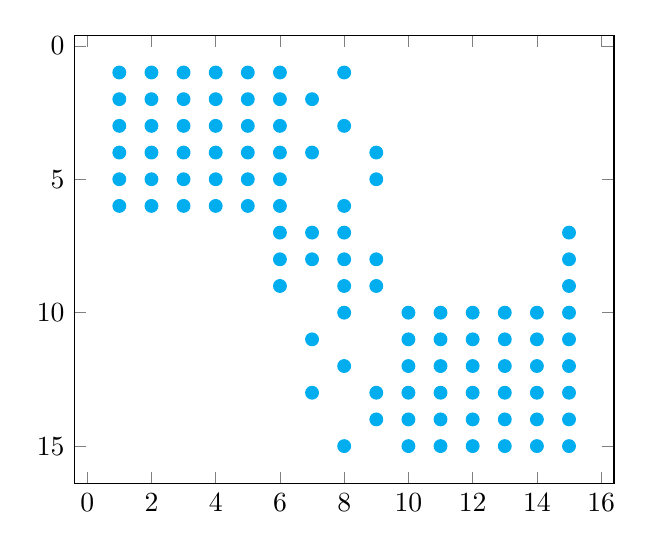
\begin{tikzpicture}

\begin{axis}[%
%width=4.52083333333333in,
%height=3.565625in,
%scale only axis,
%xmin=0,
%xmax=16,
%xlabel={nz = 99},
y dir=reverse,
%ymin=0,
%ymax=16
]
\addplot [
color=cyan,
mark size=2.3pt,
only marks,
mark=*,
mark options={solid},
forget plot
]
table[row sep=crcr]{
1 1\\ 2 1\\ 3 1\\ 4 1\\ 5 1\\ 6 1\\ 8 1\\ 
%
1 2\\ 2 2\\ 3 2\\ 4 2\\ 5 2\\ 6 2\\ 7 2\\
%
1 3\\ 2 3\\ 3 3\\ 4 3\\ 5 3\\ 6 3\\ 8 3\\
%
1 4\\ 2 4\\ 3 4\\ 4 4\\ 5 4\\ 6 4\\ 7 4\\ 9 4 \\
%
1 5\\ 2 5\\ 3 5\\ 4 5\\ 5 5\\ 6 5\\ 9 5\\
%
1 6\\ 2 6\\ 3 6\\ 4 6\\ 5 6\\ 6 6\\ 8 6\\
%
6 7\\ 7 7\\ 8 7 \\ 15 7\\
%
6 8\\ 7 8\\ 8 8\\9 8\\ 15 8\\
%
6 9\\ 8 9 \\ 9 9\\ 15 9\\
%
8 10\\ 10 10\\ 11 10\\ 12 10\\ 13 10\\ 14 10\\ 15 10\\
%
7 11\\ 10 11\\ 11 11\\ 12 11\\ 13 11\\ 14 11\\ 15 11\\
%
8 12\\ 10 12\\ 11 12\\ 12 12\\ 13 12\\ 14 12\\ 15 12\\
%
7 13\\9 13\\ 10 13\\ 11 13\\ 12 13\\ 13 13\\ 14 13\\ 15 13\\
%
9 14\\ 10 14\\ 11 14\\ 12 14\\ 13 14\\ 14 14\\ 15 14\\
%
8 15\\ 10 15\\ 11 15\\ 12 15\\ 13 15\\ 14 15\\ 15 15\\
};
%\addplot [
%color=blue,
%mark size=2.3pt,
%only marks,
%mark=*,
%mark options={solid},
%forget plot
%]
%table[row sep=crcr]{
%8 1\\
%};
\end{axis}
\end{tikzpicture}%
\end{figure}
\begin{figure}
\centering
% This file was created by matlab2tikz v0.4.2.
% Copyright (c) 2008--2013, Nico Schlömer <nico.schloemer@gmail.com>
% All rights reserved.
% 
% The latest updates can be retrieved from
%   http://www.mathworks.com/matlabcentral/fileexchange/22022-matlab2tikz
% where you can also make suggestions and rate matlab2tikz.
% 
% 
% 
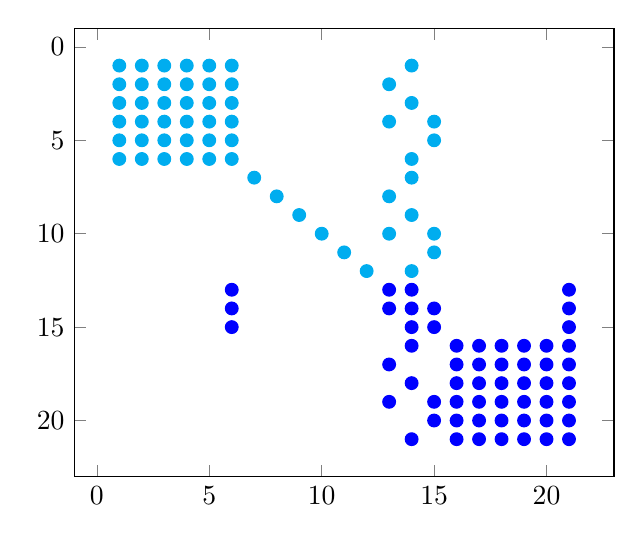
\begin{tikzpicture}

\begin{axis}[%
%width=4.52083333333333in,
%height=3.565625in,
%scale only axis,
%xmin=0,
%xmax=16,
%xlabel={nz = 99},
y dir=reverse,
%ymin=0,
%ymax=16
]
\addplot [
color=cyan,
mark size=2.3pt,
only marks,
mark=*,
mark options={solid},
forget plot
]
table[row sep=crcr]{
1 1\\ 2 1\\ 3 1\\ 4 1\\ 5 1\\ 6 1\\ 14 1\\ 
%
1 2\\ 2 2\\ 3 2\\ 4 2\\ 5 2\\ 6 2\\ 13 2\\
%
1 3\\ 2 3\\ 3 3\\ 4 3\\ 5 3\\ 6 3\\ 14 3\\
%
1 4\\ 2 4\\ 3 4\\ 4 4\\ 5 4\\ 6 4\\ 13 4\\ 15 4 \\
%
1 5\\ 2 5\\ 3 5\\ 4 5\\ 5 5\\ 6 5\\ 15 5\\
%
1 6\\ 2 6\\ 3 6\\ 4 6\\ 5 6\\ 6 6\\ 14 6\\
%
7 7\\ 14 7 \\
%
8 8\\ 13 8 \\
%
9 9\\ 14 9 \\
%
10 10\\ 13 10\\ 15 10\\
%
11 11\\ 15 11\\
%
12 12\\ 14 12\\
%
};
\addplot [
color=blue,
mark size=2.3pt,
only marks,
mark=*,
mark options={solid},
forget plot
]
table[row sep=crcr]{
6 13\\ 13 13\\ 14 13 \\ 21 13\\
%
6 14\\ 13 14\\ 14 14\\15 14\\ 21 14\\
%
6 15\\ 14 15 \\ 15 15\\ 21 15\\
%
14 16        \\ 16 16\\ 17 16\\ 18 16\\ 19 16\\ 20 16\\ 21 16\\
%
13 17        \\ 16 17\\ 17 17\\ 18 17\\ 19 17\\ 20 17\\ 21 17\\
%
14 18        \\ 16 18\\ 17 18\\ 18 18\\ 19 18\\ 20 18\\ 21 18\\
%
13 19\\ 15 19\\ 16 19\\ 17 19\\ 18 19\\ 19 19\\ 20 19\\ 21 19\\
%
15 20        \\ 16 20\\ 17 20\\ 18 20\\ 19 20\\ 20 20\\ 21 20\\
%
14 21        \\ 16 21\\ 17 21\\ 18 21\\ 19 21\\ 20 21\\ 21 21\\
};
\end{axis}
\end{tikzpicture}%
\end{figure}
\begin{figure}
\centering
% This file was created by matlab2tikz v0.4.2.
% Copyright (c) 2008--2013, Nico Schlömer <nico.schloemer@gmail.com>
% All rights reserved.
% 
% The latest updates can be retrieved from
%   http://www.mathworks.com/matlabcentral/fileexchange/22022-matlab2tikz
% where you can also make suggestions and rate matlab2tikz.
% 
% 
% 
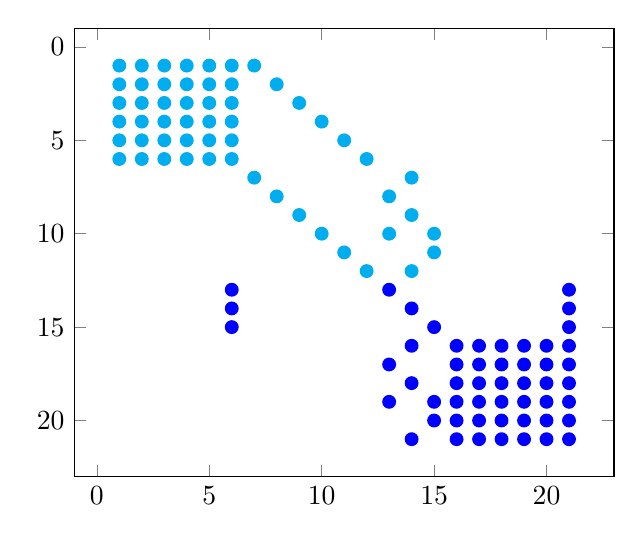
\begin{tikzpicture}

\begin{axis}[%
%width=4.52083333333333in,
%height=3.565625in,
%scale only axis,
%xmin=0,
%xmax=16,
%xlabel={nz = 99},
y dir=reverse,
%ymin=0,
%ymax=16
]
\addplot [
color=cyan,
mark size=2.3pt,
only marks,
mark=*,
mark options={solid},
forget plot
]
table[row sep=crcr]{
1 1\\ 2 1\\ 3 1\\ 4 1\\ 5 1\\ 6 1\\ 7 1\\ 
%
1 2\\ 2 2\\ 3 2\\ 4 2\\ 5 2\\ 6 2\\ 8 2\\
%
1 3\\ 2 3\\ 3 3\\ 4 3\\ 5 3\\ 6 3\\ 9 3\\
%
1 4\\ 2 4\\ 3 4\\ 4 4\\ 5 4\\ 6 4\\ 10 4\\
%
1 5\\ 2 5\\ 3 5\\ 4 5\\ 5 5\\ 6 5\\ 11 5\\
%
1 6\\ 2 6\\ 3 6\\ 4 6\\ 5 6\\ 6 6\\ 12 6\\
%
7 7\\ 14 7 \\
%
8 8\\ 13 8 \\
%
9 9\\ 14 9 \\
%
10 10\\ 13 10\\ 15 10\\
%
11 11\\ 15 11\\
%
12 12\\ 14 12\\
};
\addplot [
color=blue,
mark size=2.3pt,
only marks,
mark=*,
mark options={solid},
forget plot
]
table[row sep=crcr]{
6 13\\ 13 13\\ 21 13\\
%
6 14\\ 14 14\\ 21 14\\
%
6 15\\ 15 15\\ 21 15\\
%
14 16        \\ 16 16\\ 17 16\\ 18 16\\ 19 16\\ 20 16\\ 21 16\\
%
13 17        \\ 16 17\\ 17 17\\ 18 17\\ 19 17\\ 20 17\\ 21 17\\
%
14 18        \\ 16 18\\ 17 18\\ 18 18\\ 19 18\\ 20 18\\ 21 18\\
%
13 19\\ 15 19\\ 16 19\\ 17 19\\ 18 19\\ 19 19\\ 20 19\\ 21 19\\
%
15 20        \\ 16 20\\ 17 20\\ 18 20\\ 19 20\\ 20 20\\ 21 20\\
%
14 21        \\ 16 21\\ 17 21\\ 18 21\\ 19 21\\ 20 21\\ 21 21\\
};
\end{axis}
\end{tikzpicture}%
\end{figure}
\begin{figure}
\centering
% This file was created by matlab2tikz v0.4.2.
% Copyright (c) 2008--2013, Nico Schlömer <nico.schloemer@gmail.com>
% All rights reserved.
% 
% The latest updates can be retrieved from
%   http://www.mathworks.com/matlabcentral/fileexchange/22022-matlab2tikz
% where you can also make suggestions and rate matlab2tikz.
% 
% 
% 
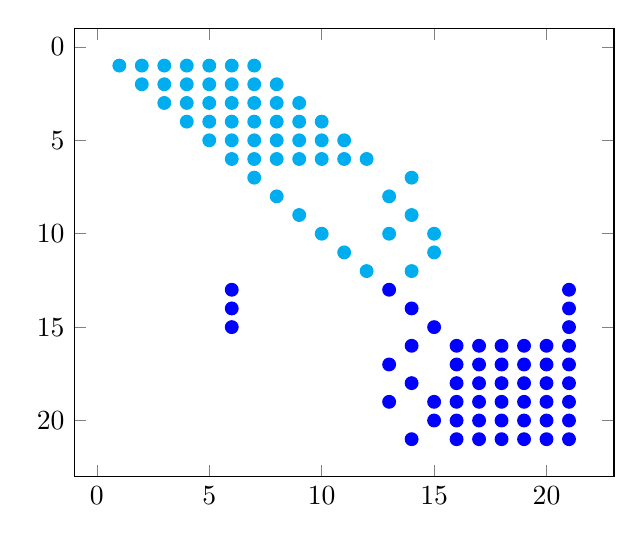
\begin{tikzpicture}

\begin{axis}[%
%width=4.52083333333333in,
%height=3.565625in,
%scale only axis,
%xmin=0,
%xmax=16,
%xlabel={nz = 99},
y dir=reverse,
%ymin=0,
%ymax=16
]
\addplot [
color=cyan,
mark size=2.3pt,
only marks,
mark=*,
mark options={solid},
forget plot
]
table[row sep=crcr]{
1 1\\ 2 1\\ 3 1\\ 4 1\\ 5 1\\ 6 1\\ 7 1\\ 
%
      2 2\\ 3 2\\ 4 2\\ 5 2\\ 6 2\\ 7 2 \\ 8 2\\
%
            3 3\\ 4 3\\ 5 3\\ 6 3\\ 7 3 \\ 8 3 \\ 9 3\\
%
                  4 4\\ 5 4\\ 6 4\\ 7 4 \\ 8 4 \\ 9 4 \\ 10 4\\
%
                        5 5\\ 6 5\\ 7 5 \\ 8 5 \\ 9 5 \\ 10 5 \\ 11 5 \\ 
%
                              6 6\\ 7 6 \\ 8 6 \\ 9 6 \\ 10 6 \\ 11 6 \\ 12 6\\
%
7 7\\ 14 7 \\
%
8 8\\ 13 8 \\
%
9 9\\ 14 9 \\
%
10 10\\ 13 10\\ 15 10\\
%
11 11\\ 15 11\\
%
12 12\\ 14 12\\
};
\addplot [
color=blue,
mark size=2.3pt,
only marks,
mark=*,
mark options={solid},
forget plot
]
table[row sep=crcr]{
6 13\\ 13 13\\ 21 13\\
%
6 14\\ 14 14\\ 21 14\\
%
6 15\\ 15 15\\ 21 15\\
%
14 16        \\ 16 16\\ 17 16\\ 18 16\\ 19 16\\ 20 16\\ 21 16\\
%
13 17        \\ 16 17\\ 17 17\\ 18 17\\ 19 17\\ 20 17\\ 21 17\\
%
14 18        \\ 16 18\\ 17 18\\ 18 18\\ 19 18\\ 20 18\\ 21 18\\
%
13 19\\ 15 19\\ 16 19\\ 17 19\\ 18 19\\ 19 19\\ 20 19\\ 21 19\\
%
15 20        \\ 16 20\\ 17 20\\ 18 20\\ 19 20\\ 20 20\\ 21 20\\
%
14 21        \\ 16 21\\ 17 21\\ 18 21\\ 19 21\\ 20 21\\ 21 21\\
};
\end{axis}
\end{tikzpicture}%
\end{figure}
\begin{figure}
\centering
% This file was created by matlab2tikz v0.4.2.
% Copyright (c) 2008--2013, Nico Schlömer <nico.schloemer@gmail.com>
% All rights reserved.
% 
% The latest updates can be retrieved from
%   http://www.mathworks.com/matlabcentral/fileexchange/22022-matlab2tikz
% where you can also make suggestions and rate matlab2tikz.
% 
% 
% 
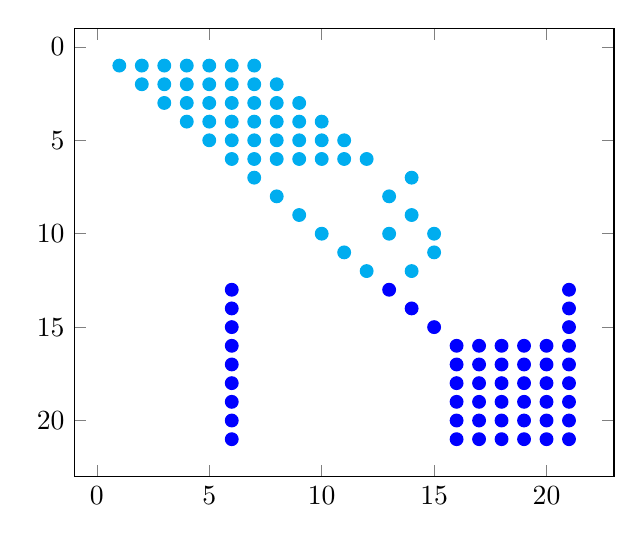
\begin{tikzpicture}

\begin{axis}[%
%width=4.52083333333333in,
%height=3.565625in,
%scale only axis,
%xmin=0,
%xmax=16,
%xlabel={nz = 99},
y dir=reverse,
%ymin=0,
%ymax=16
]
\addplot [
color=cyan,
mark size=2.3pt,
only marks,
mark=*,
mark options={solid},
forget plot
]
table[row sep=crcr]{
1 1\\ 2 1\\ 3 1\\ 4 1\\ 5 1\\ 6 1\\ 7 1\\ 
%
      2 2\\ 3 2\\ 4 2\\ 5 2\\ 6 2\\ 7 2 \\ 8 2\\
%
            3 3\\ 4 3\\ 5 3\\ 6 3\\ 7 3 \\ 8 3 \\ 9 3\\
%
                  4 4\\ 5 4\\ 6 4\\ 7 4 \\ 8 4 \\ 9 4 \\ 10 4\\
%
                        5 5\\ 6 5\\ 7 5 \\ 8 5 \\ 9 5 \\ 10 5 \\ 11 5 \\ 
%
                              6 6\\ 7 6 \\ 8 6 \\ 9 6 \\ 10 6 \\ 11 6 \\ 12 6\\
};
\addplot [
color=cyan,
mark size=2.3pt,
only marks,
mark=*,
mark options={solid},
forget plot
]
table[row sep=crcr]{
%
7 7\\ 14 7 \\
%
8 8\\ 13 8 \\
%
9 9\\ 14 9 \\
%
10 10\\ 13 10\\ 15 10\\
%
11 11\\ 15 11\\
%
12 12\\ 14 12\\
};
\addplot [
color=blue,
mark size=2.3pt,
only marks,
mark=*,
mark options={solid},
forget plot
]
table[row sep=crcr]{
6 13\\ 13 13\\ 21 13\\
%
6 14\\ 14 14\\ 21 14\\
%
6 15\\ 15 15\\ 21 15\\
%
6 16\\ 16 16\\ 17 16\\ 18 16\\ 19 16\\ 20 16\\ 21 16\\
%
6 17\\ 16 17\\ 17 17\\ 18 17\\ 19 17\\ 20 17\\ 21 17\\
%
6 18\\ 16 18\\ 17 18\\ 18 18\\ 19 18\\ 20 18\\ 21 18\\
%
6 19\\ 16 19\\ 17 19\\ 18 19\\ 19 19\\ 20 19\\ 21 19\\
%
6 20\\ 16 20\\ 17 20\\ 18 20\\ 19 20\\ 20 20\\ 21 20\\
%
6 21\\ 16 21\\ 17 21\\ 18 21\\ 19 21\\ 20 21\\ 21 21\\
};
\end{axis}
\end{tikzpicture}%
\end{figure}
\begin{figure}
\centering
% This file was created by matlab2tikz v0.4.2.
% Copyright (c) 2008--2013, Nico Schlömer <nico.schloemer@gmail.com>
% All rights reserved.
% 
% The latest updates can be retrieved from
%   http://www.mathworks.com/matlabcentral/fileexchange/22022-matlab2tikz
% where you can also make suggestions and rate matlab2tikz.
% 
% 
% 
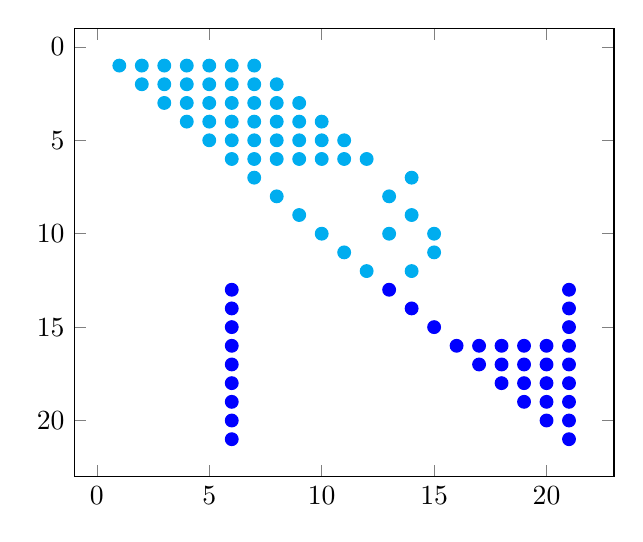
\begin{tikzpicture}

\begin{axis}[%
%width=4.52083333333333in,
%height=3.565625in,
%scale only axis,
%xmin=0,
%xmax=16,
%xlabel={nz = 99},
y dir=reverse,
%ymin=0,
%ymax=16
]
\addplot [
color=cyan,
mark size=2.3pt,
only marks,
mark=*,
mark options={solid},
forget plot
]
table[row sep=crcr]{
1 1\\ 2 1\\ 3 1\\ 4 1\\ 5 1\\ 6 1\\ 7 1\\ 
%
      2 2\\ 3 2\\ 4 2\\ 5 2\\ 6 2\\ 7 2 \\ 8 2\\
%
            3 3\\ 4 3\\ 5 3\\ 6 3\\ 7 3 \\ 8 3 \\ 9 3\\
%
                  4 4\\ 5 4\\ 6 4\\ 7 4 \\ 8 4 \\ 9 4 \\ 10 4\\
%
                        5 5\\ 6 5\\ 7 5 \\ 8 5 \\ 9 5 \\ 10 5 \\ 11 5 \\ 
%
                              6 6\\ 7 6 \\ 8 6 \\ 9 6 \\ 10 6 \\ 11 6 \\ 12 6\\
};
\addplot [
color=cyan,
mark size=2.3pt,
only marks,
mark=*,
mark options={solid},
forget plot
]
table[row sep=crcr]{
%
7 7\\ 14 7 \\
%
8 8\\ 13 8 \\
%
9 9\\ 14 9 \\
%
10 10\\ 13 10\\ 15 10\\
%
11 11\\ 15 11\\
%
12 12\\ 14 12\\
};
\addplot [
color=blue,
mark size=2.3pt,
only marks,
mark=*,
mark options={solid},
forget plot
]
table[row sep=crcr]{
6 13\\ 13 13\\ 21 13\\
%
6 14\\ 14 14\\ 21 14\\
%
6 15\\ 15 15\\ 21 15\\
%
6 16\\ 16 16\\ 17 16\\ 18 16\\ 19 16\\ 20 16\\ 21 16\\
%
6 17\\         17 17\\ 18 17\\ 19 17\\ 20 17\\ 21 17\\
%
6 18\\                 18 18\\ 19 18\\ 20 18\\ 21 18\\
%
6 19\\                         19 19\\ 20 19\\ 21 19\\
%
6 20\\                                 20 20\\ 21 20\\
%
6 21\\                                         21 21\\
};
\end{axis}
\end{tikzpicture}%
\end{figure}
\begin{figure}
\centering
% This file was created by matlab2tikz v0.4.2.
% Copyright (c) 2008--2013, Nico Schlömer <nico.schloemer@gmail.com>
% All rights reserved.
% 
% The latest updates can be retrieved from
%   http://www.mathworks.com/matlabcentral/fileexchange/22022-matlab2tikz
% where you can also make suggestions and rate matlab2tikz.
% 
% 
% 
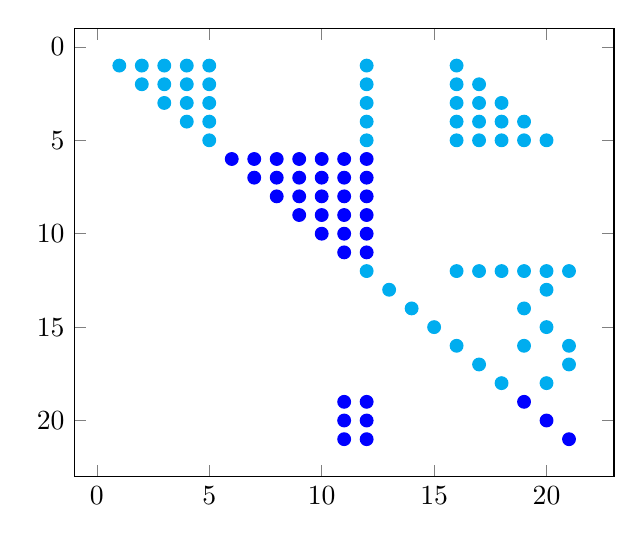
\begin{tikzpicture}

\begin{axis}[%
%width=4.52083333333333in,
%height=3.565625in,
%scale only axis,
%xmin=0,
%xmax=16,
%xlabel={nz = 99},
y dir=reverse,
%ymin=0,
%ymax=16
]
\addplot [
color=cyan,
mark size=2.3pt,
only marks,
mark=*,
mark options={solid},
forget plot
]
table[row sep=crcr]{
1 1\\ 2 1\\ 3 1\\ 4 1\\ 5 1\\ 12 1\\ 16 1\\ 
%
      2 2\\ 3 2\\ 4 2\\ 5 2\\ 12 2\\ 16 2 \\ 17 2\\
%
            3 3\\ 4 3\\ 5 3\\ 12 3\\ 16 3 \\ 17 3 \\ 18 3\\
%
                  4 4\\ 5 4\\ 12 4\\ 16 4 \\ 17 4 \\ 18 4 \\ 19 4\\
%
                        5 5\\ 12 5\\ 16 5 \\ 17 5 \\ 18 5 \\ 19 5 \\ 20 5 \\ 
%
                              12 12\\ 16 12 \\ 17 12 \\ 18 12 \\ 19 12 \\ 20 12 \\ 21 12 \\ 
};
\addplot [
color=cyan,
mark size=2.3pt,
only marks,
mark=*,
mark options={solid},
forget plot
]
table[row sep=crcr]{
%
13 13 \\         20 13 \\
%
14 14 \\ 19 14 \\
%
15 15 \\         20 15\\
%
16 16 \\ 19 16\\         21 16\\
%
17 17 \\                 21 17\\
%
18 18 \\         20 18\\
};
\addplot [
color=blue,
mark size=2.3pt,
only marks,
mark=*,
mark options={solid},
forget plot
]
table[row sep=crcr]{
11 19\\ 12 19\\ 19 19\\
%
11 20\\ 12 20\\ 20 20\\
%
11 21\\ 12 21\\ 21 21\\
%
12 6 \\ 6 6\\ 7 6\\ 8 6\\ 9 6\\ 10 6 \\ 11 6 \\
%
12 7 \\       7 7\\ 8 7\\ 9 7\\ 10 7 \\ 11 7 \\
%
12 8 \\             8 8\\ 9 8\\ 10 8 \\ 11 8 \\
%
12 9 \\                   9 9\\ 10 9 \\ 11 9 \\
%
12 10\\                         10 10\\ 11 10\\
%
12 11\\                                 11 11\\
};
\end{axis}
\end{tikzpicture}%
\end{figure}
\begin{figure}
\centering
% This file was created by matlab2tikz v0.4.2.
% Copyright (c) 2008--2013, Nico Schlömer <nico.schloemer@gmail.com>
% All rights reserved.
% 
% The latest updates can be retrieved from
%   http://www.mathworks.com/matlabcentral/fileexchange/22022-matlab2tikz
% where you can also make suggestions and rate matlab2tikz.
% 
% 
% 
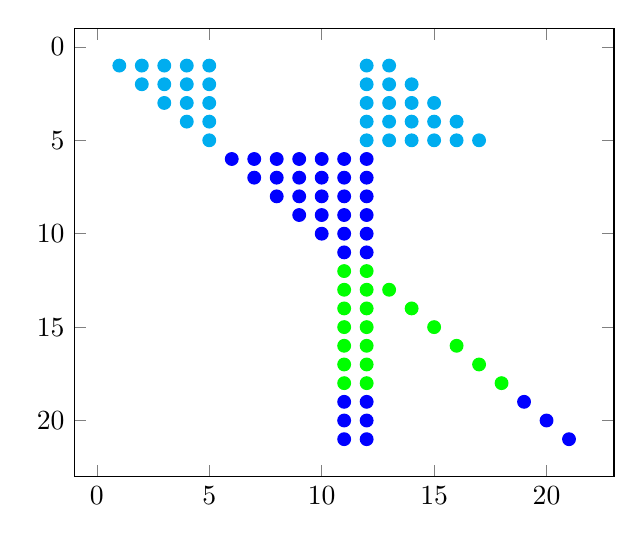
\begin{tikzpicture}

\begin{axis}[%
%width=4.52083333333333in,
%height=3.565625in,
%scale only axis,
%xmin=0,
%xmax=16,
%xlabel={nz = 99},
y dir=reverse,
%ymin=0,
%ymax=16
]
\addplot [
color=cyan,
mark size=2.3pt,
only marks,
mark=*,
mark options={solid},
forget plot
]
table[row sep=crcr]{
1 1\\ 2 1\\ 3 1\\ 4 1\\ 5 1\\ 12 1\\ 13 1\\ 
%
      2 2\\ 3 2\\ 4 2\\ 5 2\\ 12 2\\ 13 2 \\ 14 2\\
%
            3 3\\ 4 3\\ 5 3\\ 12 3\\ 13 3 \\ 14 3 \\ 15 3\\
%
                  4 4\\ 5 4\\ 12 4\\ 13 4 \\ 14 4 \\ 15 4 \\ 16 4\\
%
                        5 5\\ 12 5\\ 13 5 \\ 14 5 \\ 15 5 \\ 16 5 \\ 17 5 \\ 
};
\addplot [
color=green,
mark size=2.3pt,
only marks,
mark=*,
mark options={solid},
forget plot
]
table[row sep=crcr]{
11 12 \\ 12 12\\
%
11 13 \\ 12 13 \\ 13 13 \\
%
11 14 \\ 12 14 \\ 14 14 \\
%
11 15 \\ 12 15 \\ 15 15 \\
%
11 16 \\ 12 16 \\ 16 16 \\
%
11 17 \\ 12 17 \\ 17 17 \\
%
11 18 \\ 12 18 \\ 18 18 \\
};
\addplot [
color=blue,
mark size=2.3pt,
only marks,
mark=*,
mark options={solid},
forget plot
]
table[row sep=crcr]{
11 19\\ 12 19\\ 19 19\\
%
11 20\\ 12 20\\ 20 20\\
%
11 21\\ 12 21\\ 21 21\\
%
12 6 \\ 6 6\\ 7 6\\ 8 6\\ 9 6\\ 10 6 \\ 11 6 \\
%
12 7 \\       7 7\\ 8 7\\ 9 7\\ 10 7 \\ 11 7 \\
%
12 8 \\             8 8\\ 9 8\\ 10 8 \\ 11 8 \\
%
12 9 \\                   9 9\\ 10 9 \\ 11 9 \\
%
12 10\\                         10 10\\ 11 10\\
%
12 11\\                                 11 11\\
};
\end{axis}
\end{tikzpicture}%
\end{figure}
\begin{figure}
\centering
% This file was created by matlab2tikz v0.4.2.
% Copyright (c) 2008--2013, Nico Schlömer <nico.schloemer@gmail.com>
% All rights reserved.
% 
% The latest updates can be retrieved from
%   http://www.mathworks.com/matlabcentral/fileexchange/22022-matlab2tikz
% where you can also make suggestions and rate matlab2tikz.
% 
% 
% 
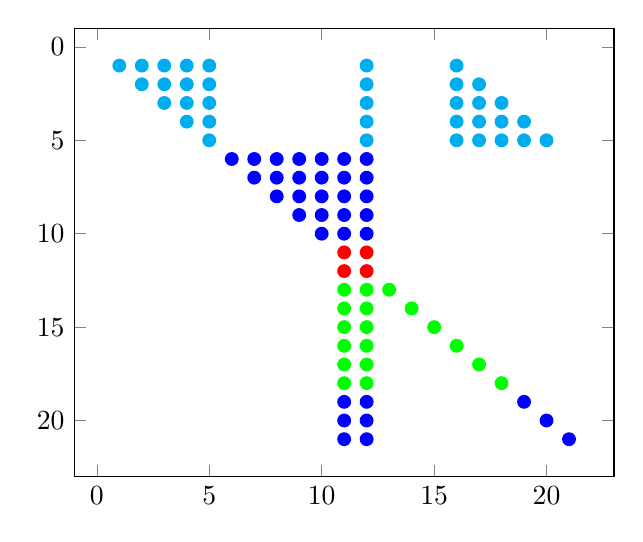
\begin{tikzpicture}

\begin{axis}[%
%width=4.52083333333333in,
%height=3.565625in,
%scale only axis,
%xmin=0,
%xmax=16,
%xlabel={nz = 99},
y dir=reverse,
%ymin=0,
%ymax=16
]
\addplot [
color=cyan,
mark size=2.3pt,
only marks,
mark=*,
mark options={solid},
forget plot
]
table[row sep=crcr]{
1 1\\ 2 1\\ 3 1\\ 4 1\\ 5 1\\ 12 1\\ 16 1\\ 
%
      2 2\\ 3 2\\ 4 2\\ 5 2\\ 12 2\\ 16 2 \\ 17 2\\
%
            3 3\\ 4 3\\ 5 3\\ 12 3\\ 16 3 \\ 17 3 \\ 18 3\\
%
                  4 4\\ 5 4\\ 12 4\\ 16 4 \\ 17 4 \\ 18 4 \\ 19 4\\
%
                        5 5\\ 12 5\\ 16 5 \\ 17 5 \\ 18 5 \\ 19 5 \\ 20 5 \\ 
};
\addplot [
color=green,
mark size=2.3pt,
only marks,
mark=*,
mark options={solid},
forget plot
]
table[row sep=crcr]{
11 13 \\ 12 13 \\ 13 13 \\
%
11 14 \\ 12 14 \\ 14 14 \\
%
11 15 \\ 12 15 \\ 15 15 \\
%
11 16 \\ 12 16 \\ 16 16 \\
%
11 17 \\ 12 17 \\ 17 17 \\
%
11 18 \\ 12 18 \\ 18 18 \\
};
\addplot [
color=red,
mark size=2.3pt,
only marks,
mark=*,
mark options={solid},
forget plot
]
table[row sep=crcr]{
11 11 \\ 12 11\\
%
11 12\\  12 12\\
};
\addplot [
color=blue,
mark size=2.3pt,
only marks,
mark=*,
mark options={solid},
forget plot
]
table[row sep=crcr]{
11 19\\ 12 19\\ 19 19\\
%
11 20\\ 12 20\\ 20 20\\
%
11 21\\ 12 21\\ 21 21\\
%
12 6 \\ 6 6\\ 7 6\\ 8 6\\ 9 6\\ 10 6 \\ 11 6 \\
%
12 7 \\       7 7\\ 8 7\\ 9 7\\ 10 7 \\ 11 7 \\
%
12 8 \\             8 8\\ 9 8\\ 10 8 \\ 11 8 \\
%
12 9 \\                   9 9\\ 10 9 \\ 11 9 \\
%
12 10\\                         10 10\\ 11 10\\
};
\end{axis}
\end{tikzpicture}%
\end{figure}



\end{document}